\documentclass{sig-alternate-05-2015}
\begin{document}

\setcopyright{acmcopyright}

\title{Improving Collaborative Filtering with Pseudo Side Information}

\numberofauthors{1}
\author{
\alignauthor
Chao Lv \quad
Lili Yao \quad
Yansong Feng \quad
Dongyan Zhao\titlenote{Corresponding author.}\\
\affaddr{Institute of Computer Science and Technology}\\
\affaddr{Peking University, Beijing 100871, China}\\
\email{\{lvchao, yaolili, fengyansong, zhaodongyan\}@pku.edu.cn}
}

\maketitle

\begin{abstract}
Collaborative filtering (CF) has been widely employed within recommender systems in many real-world situations.
Its basic assumption is that items liked by the same user would be similar or users like same items would share similar interest.
But it not always holds because users' interest may change over time.
If user likes two items at the same time period, there is a strong possibility that they are similar.
But the possibility will become small if user likes they at different time point.
In this paper, we propose a method that takes advantage of user ratings timeline to describe the time sensitive relationship between users and items.
To reach this goal, we use a language-based algorithm to learn effective latent embeddings for users and items.
Language model aims to extract the potential association between sentences and words, which is similar with users and items in recommender system.
The learned embedding for users and items can be considered as a kind of side information that describes the time sensitive relationship between users and items.
We then combine them with origin rating information to predict missing ratings in a feature-based collaborative filtering framework.
Experimental results on three MovieLens datasets demonstrate that our approach can achieve the state-of-the-art performance.
\end{abstract}

\category{H.2.8}{Database Management}{Data Mining}
\category{H.3.3}{Information Search and Retrieval}{Information Filtering}
\terms{Algorithms, Experimentation, Performance}
\keywords{Recommender System; Collaborative Filtering; Embedding Model;}

\section{Introduction}
Recommender system has become more and more popular in many real-world situations, in the modern era of information overload.
Lots of websites (e.g. Amazon, Netflix, Alibaba and Hulu) use recommender system to target customers and provide them with useful information.
Recommender system aims to help users find the items, they are more likely to be interested in, from huge amounts of candidates.
A widely used setting of recommendation system is to predict how a user would rate an item (such as a movie) given the past rating history of the users.
Many classical recommendation methods have been proposed in recent years and they can be categorized into three classes:
content-based methods, collaborative filtering (CF) based methods, and hybrid methods.
Content-based methods \cite{pazzani2007content} make use of user profiles or product descriptions for recommendation.
CF-based methods \cite{su2009survey} use the past activities or preferences, such as user ratings on items, without using user or product content information.
Hybrid methods \cite{wang2011collaborative} seek to get the best of both worlds by combining content-based and CF-based methods.
The CF based methods have been developed for many years and keep to be a hot area in both academia and industry due to their impressive performance.
Collaborative filtering focuses on predicting the preference of one user by combining his feedback on a few items and the feedback of all other users.
Among various CF based methods, matrix factorization (MF) models have become popular and achieves the state-of-the-art performance \cite{koren2009matrix}.

\section{Relate Work}
\subsection{Matrix Factoriztion}
\subsection{Nerual Network}

\section{Our Approach}
In this section,
we first introduce our embedding framework to extract the relationship
between users and items based on the local interest and global interest.
Then we treat the embeding information as pseudo side information,
and utilize it in the feature-based matrix factorization.

\subsection{Embedding Model}
As we know, users' interest changes over time,
but in a fixed time period, their interest should be stable.
We define the interest in a fixed time period as \textbf{local interest}
and the interest in a long time period as \textbf{global interest}.
It is common that the items in the same time period
should have a higher possibility to be similar than
items not in the same time period.

\begin{figure*}[htbp]
	\centering
	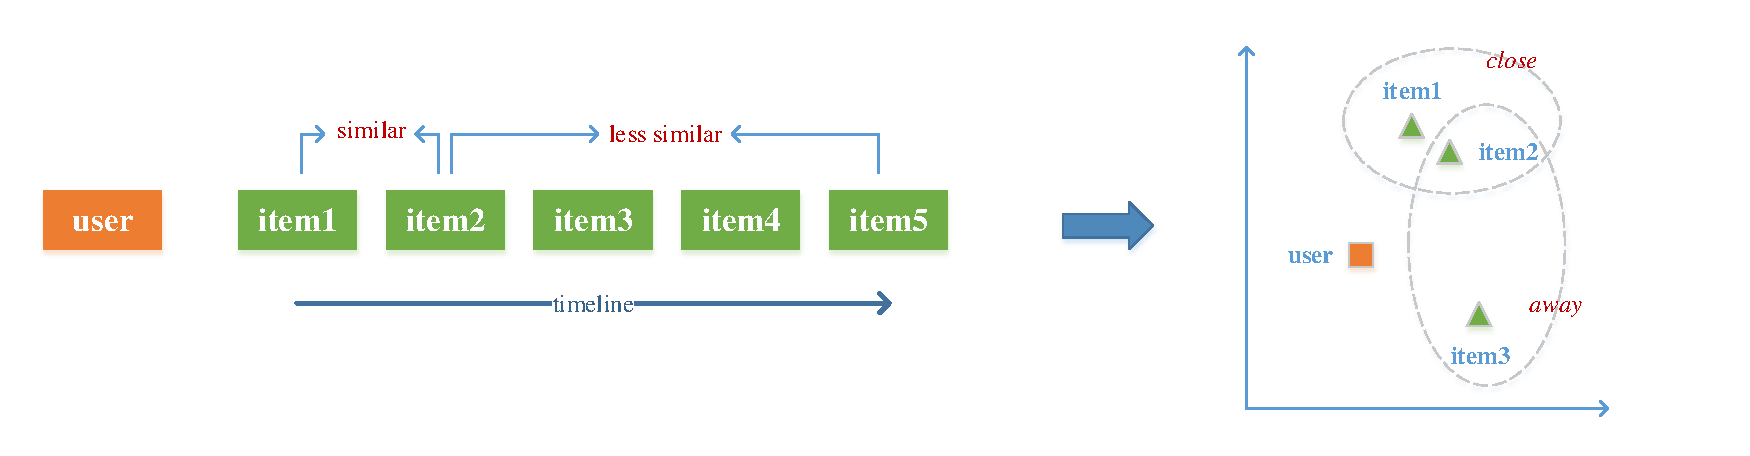
\includegraphics[scale=0.6]{images/1.pdf}
	\caption{A Example for Local Interest and Global Interest}
	\label{fig:example}
\end{figure*}

For example, as illustrated in the left of Figure \ref{fig:example},
for a cetain $user$, five items, he interacted in the last,
are listed on the timeline according to the time order.
$item_2$ is more close to $item_1$ than $item_5$,
so it shoule be more similar with $item_1$ than $item_5$.
\footnote{We use time window to judge time proximity instead of extract timestamp here for convenience.}

By embedding model, we want to project users and items in a low-dimensionality space,
and change the interest similarity into sapce distance.
$item_2$ and $item_1$ are close to each other than $item_2$ and $item_5$
in the projection space, as shown in the right of Figure \ref{fig:example}.

Inspired by paragraph2vec algorithm \cite{le2014distributed} for learning vector representations of words
which take advantage of a word order observed in a sentence,
we choose to use neural network based language model
to embed this interest similarity information.

\begin{figure}[htbp]
	\centering
	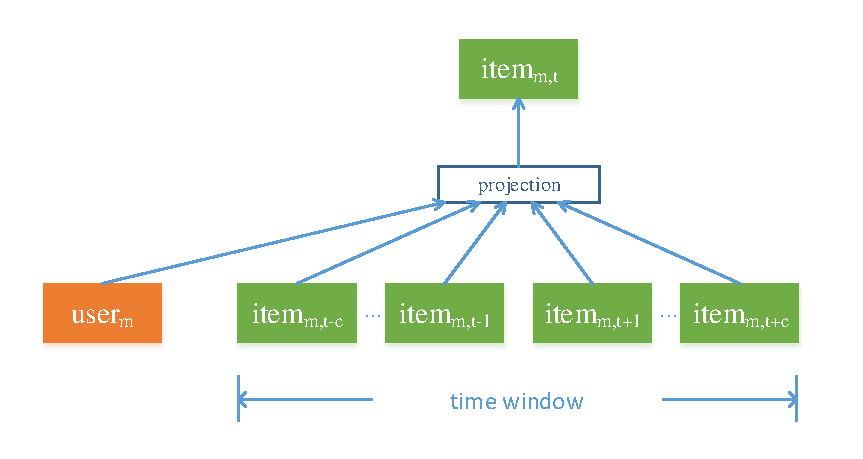
\includegraphics[scale=0.55]{images/2.pdf}
	\caption{Embedding Model for Extracting Interest Similarity from Users and Items}
	\label{fig:embedding}
\end{figure}

The embedding model simultaneously learns vector representations of users and items
by considering the user as a global context,
and the architecture of the embedding model is illustrated in Figure \ref{fig:embedding}.
The training data set was derived from users interaction timeline $T$,
which comprises users $u_n$ and their interacted items
ordered by the interacted time,
$i_{n_1}, i_{n_2}, ..., i_{n_{L_n}}$,
where $L_n$ denotes number of items interacted by user $u_n$.

More formally, objective of the embedding model is to
maximize the log-likelihood over the set of $T$ of all the interaction timeline,

\begin{equation}
\begin{aligned}
	\sum^{T} &\bigg( p(u_n | i_{n_1}, i_{n_2}, ..., i_{n_{L_n}}) + \\
			 &\sum_{j=1}^{L_n} p(i_{n_j} | i_{n_{j-c}}, ..., i_{n_{j-1}}, i_{n_{j+1}},..., i_{n_{j+c}}, u_n) \bigg)
\end{aligned}
\end{equation}

where $c$ is the time window size.

$p(u_n | i_{n_1}, i_{n_2}, ..., i_{n_{L_n}})$ can be treated as predicting the global interest,
and it is defined using a softmax funxtion,

\begin{equation}
\begin{aligned}
	p(u_n | i_{n_1}, i_{n_2}, ..., i_{n_{L_n}}) =
	\frac
	{
		exp( \overline{v}_{1}^{\mathrm{T}} v_{u_n}^{'} )
	}
	{
		\sum_{i=1}^{V} exp( \overline{v}_{1}^{\mathrm{T}} v_{i}^{'} )
	}
\end{aligned}
\end{equation}

where $v_{u_n}^{'}$ is the output vector representation of $u_n$,
and $\overline{v}_{1}$ is averaged input vector representation of all the items
interacted by user $u_n$.

\begin{equation}
\begin{aligned}
	\overline{v}_{1} = \frac{\sum_{j=1}^{T_n} v_{i_{n_j}}}{T_n}
\end{aligned}
\end{equation}

Similarly, $p(i_{n_j} | i_{n_{j-c}}, ..., i_{n_{j-1}}, i_{n_{j+1}},..., i_{n_{j+c}}, u_n)$
can be treated as predict each items in the same local interest,
and it is also defined using a softmax funxtion,

\begin{equation}
\begin{aligned}
	p(i_{n_j} | i_{n_{j-c}}, ..., i_{n_{j-1}}, i_{n_{j+1}},..., i_{n_{j+c}}, u_n) =
	\frac
	{
		exp( \overline{v}_{2}^{\mathrm{T}} v_{i_{n_j}}^{'} )
	}
	{
		\sum_{i=1}^{V} exp( \overline{v}_{2}^{\mathrm{T}} v_{i}^{'} )
	}
\end{aligned}
\end{equation}

where $v_{i_{n_j}}^{'}$ is the output vector representation of $i_{n_j}$,
and $\overline{v}_{2}$ is averaged input vector representation of items in the time window
and corresponding $u_n$.

\begin{equation}
\begin{aligned}
	\overline{v}_{2} = \frac{ v_{i_{n_{j-c}}} + ... + v_{i_{n_{j-1}}} + 
	v_{i_{n_{j+1}}} + ... + v_{i_{n_{j+c}}} + v_{u_n} }{2c+1}
\end{aligned}
\end{equation}


\subsection{Learning Model}
With the help of embedding model, we can get the vector representation of users and tiems.


we use \cite{chen2012svdfeature}.


\section{Experiment}
In this section, we conduct several experiments to evaluate the effectiveness of our embedding model.
In these experiments, we also conduct corresponding analysis to investigate:
(1) the influence of the various feedback entity model parameter settings on
retrieval performance;
(2) the effects of feedback tweets number;
(3) the influence of the interpolation coefficient in query expansion and
(4) a comparison of two different entity feedback acquisition methods.



\begin{table*}[htpb]
	\centering
	\caption{Statistics of datasets used in our experiment.}
	\label{tab:topics}
	\begin{tabular}{|l|c|c|c|c|c|c|}
		\hline
		\textbf{Dataset} & \textbf{\#Users} & \textbf{\#Items} & \textbf{\#Ratings} & \textbf{Sparsity} & \textbf{User Features} & \textbf{Item Features} \\
		\hline
		MovieLens-1m  & 6,040   & 3,706  & 1,000,209  & 95.53\% & Gender, Age, and occupation & Genres \\
		MovieLens-10m & 69,878  & 10,677 & 10,000,054 & 98.66\% & - & Genres \\
		MovieLens-20m & 138,493 & 26,744 & 20,000,263 & 99.46\% & - & Genres \\
		\hline
	\end{tabular}
\end{table*}



We employ the root mean squared error (RMSE) and mean absolute error (MAE) as the evaluation metric.
RMSE and MAE are defined as:
$$ RSME = \sqrt{ \frac{1}{N} \sum_{i,j} I_{ij} (R_{ij} - \hat{R}_{ij})^2 } $$
$$ MAE = \frac{1}{N} \sum_{i,j} I_{ij} |R_{ij} - \hat{R}_{ij}| $$
where $N$ is the total number of ratings in the test set,
$R_{ij}$ is the ground-truth rating of user $i$ for item $j$,
$\hat{R_{ij}}$ denotes the corresponding predicted rating,
and $I_{ij}$ is abinary matrix that indicates the ratings in the test set.




\section{Conclusions}
This is the abstract about the paper this is the abstract about the paper.
This is the abstract about the paper this is the abstract about the paper.
This is the abstract about the paper this is the abstract about the paper.
This is the abstract about the paper this is the abstract about the paper.

\section{Acknowledgments}
The work reported in this paper is supported by the National Natural Science Foundation of China Grant 61370116.
We thank anonymous reviewers for their beneficial comments.
We also thank Feifan Fan and Yue Fei for valuable suggestions related to this paper.

\bibliographystyle{abbrv}
\bibliography{sigproc}

\end{document}
